\documentclass[12pt]{article}
\usepackage{fullpage}
\usepackage{url}
\usepackage{amsmath}
\usepackage{amsfonts}
\usepackage{algorithm}
\usepackage{algorithmic}
\usepackage{graphicx}
\usepackage{hyperref}
\usepackage{color}
\usepackage{listings}
\usepackage{verbatim}
\usepackage{enumitem}
\usepackage[parfill]{parskip}

\newcommand{\xb}{\mathbf{x}}
\newcommand{\yb}{\mathbf{y}}
\newcommand{\wb}{\mathbf{w}}
\newcommand{\Xb}{\mathbf{X}}
\newcommand{\Yb}{\mathbf{Y}}
\newcommand{\tr}{^T}
\newcommand{\hb}{\mathbf{h}}
\newcommand{\Hb}{\mathbf{H}}

\newcommand{\cmt}[1]{{\footnotesize\textcolor{red}{#1}}}
\newcommand{\todo}[1]{\cmt{TO-DO: #1}}

\newenvironment{solution}{\color{blue} \smallskip \textbf{Solution:}}{}

\title{CS294-112 Deep Reinforcement Learning HW2: \\ Policy Gradients}

\author{Hatim Ezbakhe}

\date{Monday, September 17, 2018}

\usepackage{courier}
 
\definecolor{codegreen}{rgb}{0,0.6,0}
\definecolor{codegray}{rgb}{0.5,0.5,0.5}
\definecolor{codepurple}{rgb}{0.58,0,0.82}
\definecolor{backcolour}{rgb}{0.95,0.95,0.92}

\lstdefinestyle{mystyle}{
    backgroundcolor=\color{backcolour},   
    commentstyle=\color{codegreen},
    keywordstyle=\color{magenta},
    numberstyle=\tiny\color{codegray},
    stringstyle=\color{codepurple},
    basicstyle=\footnotesize\ttfamily,
    breakatwhitespace=false,         
    breaklines=true,                 
    captionpos=b,                    
    keepspaces=true,                 
    %numbers=left,                    
    numbersep=5pt,                  
    showspaces=false,                
    showstringspaces=false,
    showtabs=false,                  
    tabsize=2
}

\lstset{style=mystyle}

\begin{document}


\maketitle

\section{Introduction}
The goal of this assignment is to experiment with policy gradient and its variants, including variance reduction methods. Your goals will be to set up policy gradient for both continuous and discrete environments and experiment with variance reduction tricks, including implementing reward-to-go and neural network baselines.

Turn in your report and code for the full homework as described in Problem 2 by September 19, 2018.

\section{Review}
Recall that the reinforcement learning objective is to learn a $\theta^*$ that maximizes the objective function:
\begin{align} \label{objective}
J(\theta) = \mathbb{E}_{\tau \sim \pi_\theta(\tau)} \left[r(\tau)\right]
\end{align}
where 
$$\pi_\theta(\tau) = p(s_1, a_1, ..., s_T, a_T) = p(s_1)\pi_\theta(a_1|s_1) \prod_{t=2}^T p(s_t | s_{t-1}, a_{t-1}) \pi_\theta(a_t | s_t)$$
and 
$$r(\tau) = r(s_1, a_1, ..., s_T, a_T) = \sum_{t=1}^T r(s_t, a_t).$$

The policy gradient approach is to directly take the gradient of this objective:
\begin{align}
\nabla_\theta J(\theta) &= \nabla_\theta \int \pi_\theta(\tau) r(\tau) d\tau \label{policygradientintegral} \\ 
&= \int \pi_\theta(\tau) \nabla_\theta \log \pi_\theta(\tau) r(\tau) d\tau. \label{scorefunctionpg}
\end{align}
In practice, the expectation over trajectories $\tau$ can be approximated from a batch of $N$ sampled trajectories:
\begin{align}
\nabla_\theta J(\theta) &\approx \frac{1}{N} \sum_{i=1}^N \nabla_\theta \log \pi_\theta(\tau_i) r(\tau_i) \\
&= \frac{1}{N} \sum_{i=1}^N \left(\sum_{t=1}^T \nabla_\theta \log \pi_\theta(a_{it} | s_{it})\right)\left(\sum_{t=1}^T r(s_{it}, a_{it})\right). \label{estimatedscorefunctionpg}
\end{align}
Here we see that the policy $\pi_\theta$ is a probability distribution over the action space, conditioned on the state. In the agent-environment loop, the agent samples an action $a_t$ from $\pi_\theta(\cdot | s_t)$ and the environment responds with a reward $r(s_t, a_t)$.

One way to reduce the variance of the policy gradient is to exploit causality: the notion that the policy cannot affect rewards in the past, yielding following the modified objective, where the sum of rewards here is a sample estimate of the $Q$ function, known as the ``reward-to-go:''
\begin{align}
\nabla_\theta J(\theta) &\approx \frac{1}{N} \sum_{i=1}^N \sum_{t=1}^T \nabla_\theta \log \pi_\theta(a_{it} | s_{it})\left(\sum_{t'=t}^T r(s_{it'}, a_{it'})\right).
\end{align}

Multiplying a discount factor $\gamma$ to the rewards can be interpreted as encouraging the agent to focus on rewards closer in the future, which can also be thought of as a means for reducing variance (because there is more variance possible futures further into the future). We saw in lecture that the discount factor can be incorporated in two ways.

The first way applies the discount on the rewards from full trajectory:
\begin{align} \label{discount_full}
\nabla_\theta J(\theta) &\approx \frac{1}{N} \sum_{i=1}^N \left(\sum_{t=1}^T \nabla_\theta \log \pi_\theta(a_{it} | s_{it})\right)\left(\sum_{t=1}^T \gamma^{t-1} r(s_{it}, a_{it})\right)
\end{align}
and the second way applies the discount on the ``reward-to-go:''
\begin{align} \label{discount_rtg}
\nabla_\theta J(\theta) &\approx \frac{1}{N} \sum_{i=1}^N \sum_{t=1}^T \nabla_\theta \log \pi_\theta(a_{it} | s_{it})\left(\sum_{t'=t}^T \gamma^{t'-t} r(s_{it'}, a_{it'})\right).
\end{align}.

We have seen in lecture that subtracting a baseline that is a constant with respect to $\tau$ from the sum of rewards
\begin{align} \label{constant_wrt_tau}
\nabla_\theta J(\theta) = \nabla_\theta \mathbb{E}_{\tau \sim \pi_\theta(\tau)} \left[r(\tau) - b\right]\
\end{align}
leaves the policy gradient unbiased because $$\nabla_\theta \mathbb{E}_{\tau \sim \pi_\theta(\tau)} \left[b\right] = \mathbb{E}_{\tau \sim \pi_\theta(\tau)} \left[\nabla_\theta \log \pi_\theta(\tau) \cdot b\right] = 0.$$

In this assignment, we will implement a value function $V_\phi^\pi$ which acts as a \textit{state-dependent} baseline. The value function is trained to approximate the sum of future rewards starting from a particular state:
\begin{align}
V_\phi^\pi(s_t) \approx \sum_{t'=t}^T \mathbb{E}_{\pi_\theta} \left[r(s_{t'}, a_{t'}) | s_t\right],
\end{align}
so the approximate policy gradient now looks like this:
\begin{align} \label{state_dependent_baseline}
\nabla_\theta J(\theta) &\approx \frac{1}{N} \sum_{i=1}^N \sum_{t=1}^T \nabla_\theta \log \pi_\theta(a_{it} | s_{it})\left(\left(\sum_{t'=t}^T \gamma^{t'-t} r(s_{it'}, a_{it'})\right) - V_\phi^\pi\left(s_{it}\right)\right).
\end{align}

\textbf{Problem 1. State-dependent baseline:}
In lecture we saw that the policy gradient is unbiased if the baseline is a constant with respect to $\tau$ (Equation~\ref{constant_wrt_tau}). The purpose of this problem is to help convince ourselves that subtracting a state-dependent baseline from the return keeps the policy gradient unbiased. For clarity we will use $p_\theta(\tau)$ instead of $\pi_\theta(\tau)$, although they mean the same thing. Using the \href{https://en.wikipedia.org/wiki/Law_of_total_expectation}{\textcolor{blue}{law of iterated expectations}} we will show that the policy gradient is still unbiased if the baseline $b$ is function of a state at a particular timestep of $\tau$ (Equation~\ref{state_dependent_baseline}). Recall from equation \ref{scorefunctionpg} that the policy gradient can be expressed as
\begin{align*}
&\mathbb{E}_{\tau \sim p_\theta(\tau)} \left[\nabla_\theta \log p_\theta(\tau)r(\tau)\right].
\end{align*}
By breaking up $p_\theta(\tau)$ into dynamics and policy terms, we can discard the dynamics terms, which are not functions of $\theta$:
\begin{align*}
&\mathbb{E}_{\tau \sim p_\theta(\tau)} \left[\sum_{t=1}^T \nabla_\theta \log \pi_\theta(a_t|s_t) \left(\sum_{t'=1}^T r(s_{t'}, a_{t'})\right)\right].
\end{align*}
When we subtract a state dependent baseline $b(s_t)$ (recall equation \ref{state_dependent_baseline}) we get
\begin{align*}
\mathbb{E}_{\tau \sim p_\theta(\tau)} \left[\sum_{t=1}^T \nabla_\theta \log \pi_\theta(a_t|s_t) \left(\left(\sum_{t'=1}^T r(s_{t'}, a_{t'})\right) - b(s_t)\right)\right].
\end{align*}
Our goal for this problem is to show that 
\begin{align*}
\mathbb{E}_{\tau \sim p_\theta(\tau)} \left[\sum_{t=1}^T \nabla_\theta \log \pi_\theta(a_t|s_t) b(s_t)\right] = 0.
\end{align*}
By \href{https://brilliant.org/wiki/linearity-of-expectation/}{\textcolor{blue}{linearity of expectation}} we can consider each term in this sum independently, so we can equivalently show that
\begin{align} \label{independent}
\sum_{t=1}^T \mathbb{E}_{\tau \sim p_\theta(\tau)}\left[ \nabla_\theta \log \pi_\theta(a_t|s_t) \left(b(s_t)\right)\right] = 0.
\end{align}
\begin{enumerate} [label=(\alph*)]
\item Using the chain rule, we can express $p_\theta(\tau)$ as a product of the state-action marginal $(s_t, a_t)$ and the probability of the rest of the trajectory conditioned on $(s_t, a_t)$ (which we denote as $(\tau / s_t, a_t | s_t, a_t)$):
    \begin{align*}
        p_\theta(\tau) = p_\theta(s_t, a_t)p_\theta(\tau / s_t, a_t | s_t, a_t)
    \end{align*}
    Please show equation \ref{independent} by using the law of iterated expectations, breaking $\mathbb{E}_{\tau \sim p_\theta(\tau)}$ by decoupling the state-action marginal from the rest of the trajectory.

\begin{solution}
By using the law of iterated expectations: 


\begin{align} 
\sum_{t=1}^T \mathbb{E}_{\tau \sim p_\theta(\tau)}\left[ \nabla_\theta \log \pi_\theta(a_t|s_t) \left(b(s_t)\right)\right] 
= \sum_{t=1}^T \mathbb{E}_{\tau \sim p_\theta(s_t, a_t)}(
  \mathbb{E}_{\frac{\tau}{s_t} \sim p_\theta(\frac{\tau}{s_t}, a_t)}\left[ \nabla_\theta \log \pi_\theta(a_t|s_t) \left(b(s_t)\right) | s_t, a_t\right])
\end{align}

And, knowing the action $a_t$ and the state $s_t$, the term within the nabla operator is constant (knowing $a_t$ and $s_t$). 
\begin{align}
\mathbb{E}_{\frac{\tau}{s_t} \sim p_\theta(\frac{\tau}{s_t}, a_t)}\left[ \nabla_\theta \log \pi_\theta(a_t|s_t) \left(b(s_t)\right) | s_t, a_t\right]) = 0
\end{align}

This gives us \ref{independent}
\end{solution}




\item Alternatively, we can consider the structure of the MDP and express $p_\theta(\tau)$ as a product of the trajectory distribution up to $s_t$ (which we denote as $(s_{1:t}, a_{1:t-1})$) and the trajectory distribution after $s_t$ conditioned on the first part (which we denote as $(s_{t+1:T}, a_{t:T} | s_{1:t}, a_{1:t-1})$):
    \begin{align*}
        p_\theta(\tau) = p_\theta(s_{1:t}, a_{1:t-1}) p_\theta(s_{t+1:T}, a_{t:T} | s_{1:t}, a_{1:t-1})
    \end{align*}
\begin{enumerate}
\item Explain why, for the inner expectation, conditioning on $(s_1, a_1, ..., a_{t^*-1}, s_{t^*})$ is equivalent to conditioning only on $s_{t^*}$.

\begin{solution}
Because the state transitions of an MDP satisfies the Markov property, the transition probability has a memorylessness property and the action taken at a step t only depends on the given state at that time t, without taking into account the previous states or actions.

Consequently conditioning on $(s_1, a_1, ..., a_{t^*-1}, s_{t^*})$ is equivalent to conditioning only on $s_{t^*}$.
\end{solution}

\item Please show equation \ref{independent} by using the law of iterated expectations, breaking $\mathbb{E}_{\tau \sim p_\theta(\tau)}$ by decoupling trajectory up to $s_t$ from the trajectory after $s_t$.

\begin{solution}

$\sum_{t=1}^T \mathbb{E}_{\tau \sim p_\theta(\tau)}\left[ \nabla_\theta \log \pi_\theta(a_t|s_t) \left(b(s_t)\right)\right] 
= \sum_{t=1}^T \mathbb{E}_{\tau \sim p_\theta(s_{1:t}, a_{1:t-1})}(
\mathbb{E}_{\frac{\tau}{s_t} \sim p_\theta(s_{t+1:T}, a_{t:T})}\left[ \nabla_\theta \log \pi_\theta(a_t|s_t) \left(b(s_t)\right) | s_{t^*}\right])$

Computing the inner expectation, using the convenient identity along a trajectory we saw in class ($\pi_\theta(\tau)\nabla_\theta \log \pi_\theta(\tau) = \nabla_\theta \pi_\theta(\tau) $):

\begin{align}
\mathbb{E}_{\frac{\tau}{s_t} \sim p_\theta(s_{t+1:T}, a_{t:T})}\left[ \nabla_\theta \log \pi_\theta(a_t|s_t) \left(b(s_t)\right) | s_{t^*}\right]) = \int \pi_\theta(\frac{a_t}{s_t}) \nabla_\theta \log \pi_\theta(a_t|s_t) b(s_t)
=  b(s_t) \nabla_\theta \int \pi_\theta(a_t|s_t)) = 0
\end{align}

\end{solution}

\end{enumerate}
\end{enumerate}
Since the policy gradient with respect to $\theta$ can be decoupled as a summation of terms over timesteps $t \in [1, T]$, because we have shown that the policy gradient is unbiased for each of these terms,
the entire policy gradient is also unbiased with respect to a vector of state-dependent baselines over the timesteps: $[b(s_1), b(s_2), ... b(s_T)]$.

\section{Code Setup}
\subsection{Files}
The starter code is available \href{https://github.com/berkeleydeeprlcourse/homework/tree/master/hw2}{\textcolor{blue}{here}}.
The only file you need to modify in this homework is \verb|train_pg_f18.py|. The files \verb|logz.py| and \verb|plots.py| are utility files; while you should look at them to understand their functionality, you will not modify them. For the Lunar Lander task, use the provided \verb|lunar_lander.py| file instead of \verb|gym/envs/box2d/lunar_lander.py|. After you fill in the appropriate methods, you should be able to just run \verb|python train_pg_f18.py| with some command line options to perform the experiments. To visualize the results, you can run \verb|python plot.py path/to/logdir|.

\subsection{Overview}
The function \verb|train_PG| is used to perform the actual training for policy gradient. The parameters passed into this function specify the algorithm's hyperparameters and environment. The \verb|Agent| class contains methods that define the computation graph, sample trajectories, estimate returns, and update the parameters of the policy.

At a high level, the dataflow of the code is structured like this:
\begin{enumerate}
    \item \textit{Build a static computation graph} in Tensorflow.
    \item \textit{Set up a Tensorflow session} to initialize the parameters of the computation graph. This is the only time you need to set up the session.
\end{enumerate}
Then we will repeat Steps 3 through 5 for $N$ iterations:
\begin{enumerate}\setcounter{enumi}{2}
    \item \textit{Sample trajectories} by executing the Tensorflow op that samples an action given an observation from the environment. Collect the states, actions, and rewards as numpy variables.
    \item \textit{Estimate returns} in numpy (estimated Q values, baseline predictions, advantages).
    \item \textit{Update parameters} by executing the Tensorflow op that updates the parameters given what you computed in Step 4.
\end{enumerate}

\section{Constructing the computation graph}

\textbf{Problem 2. Neural networks:} We will now begin to implement a neural network that parametrizes $\pi_\theta$.
\begin{enumerate} [label=(\alph*)]
\item Implement the utility function, \verb|build_mlp|, which will build a feedforward neural network with fully connected units (Hint: use \texttt{tf.layers.dense}). Test it to make sure that it produces outputs of the expected size and shape. \textbf{You do not need to include anything in your write-up about this,} it will just make your life easier.
\item Next, implement the method \verb|Agent.build_computation_graph|. At this point, you only need to implement the parts with the ``Problem 2'' header.
    \begin{enumerate} [label=(\roman*)]
        \item Define the placeholder for the advantages in \verb|Agent.define_placeholders|. We have already defined placeholders for the observations and actions. The advantages will correspond to $r(\tau)$ in the policy gradient, which may or may not include a subtracted baseline value.
        \item Create the symbolic operation \texttt{Agent.policy\_forward\_pass}: This outputs the parameters of a distribution $\pi_\theta(a|s)$. In this homework, when the distribution is over discrete actions these parameters will be the logits of a categorical distribution, and when the distribution is over continuous actions these parameters will be the mean and the log standard deviation of a multivariate Gaussian distribution. This operation will be an input to \texttt{Agent.sample\_action} and \texttt{Agent.get\_log\_prob}.
        \item Create the symbolic operation \texttt{Agent.sample\_action}: This produces a Tensorflow op, \texttt{self.sy\_sampled\_ac} that samples an action from $\pi_\theta(a|s)$. This operation will be called in \texttt{Agent.sample\_trajectories}.
        \item Create the symbolic operation \texttt{Agent.get\_log\_prob}: Given an action that the agent took in the environment, this computes the log probability of that action under $\pi_\theta(a|s)$. This will be used in the loss function.
        \item In \verb|Agent.build_computation_graph| implement a loss function (which call use the result from \texttt{Agent.get\_log\_prob}) to whose gradient is $$\nabla_\theta J(\theta) \approx \frac{1}{N} \sum_{i=1}^N \nabla_\theta \log \pi_\theta(\tau_i) r(\tau_i).$$
    \end{enumerate}
\end{enumerate}

\section{Implement Policy Gradient}
\subsection{Implementing the policy gradient loop}
\textbf{Problem 3. Policy Gradient:} Recall from lecture that an RL algorithm can viewed as consisting of three parts, which are reflected in the training loop of \verb|train_PG|:
\begin{enumerate}
    \item \verb|Agent.sample_trajectories|: Generate samples (e.g. run the policy to collect trajectories consisting of state transitions ($s, a, s', r$))
    \item \verb|Agent.estimate_return|: Estimate the return (e.g. sum together discounted rewards from the trajectories, or learn a model that predicts expected total future discounted reward)
    \item \verb|Agent.update_parameters|: Improve the policy (e.g. update the parameters of the policy with policy gradient)
\end{enumerate}
In our implementation, for clarity we will update the parameters of the value function baseline also in the third step (\verb|Agent.update_parameters|), rather than in the second step (as was described in lecture). You only need to implement the parts with the ``Problem 3'' header. 
\begin{enumerate} [label=(\alph*)]
    \item \textbf{Sample trajectories:} In \texttt{Agent.sample\_trajectories}, use the Tensorflow session to call \texttt{self.sy\_sampled\_ac} to sample an action given an observation from the environment.
    \item \textbf{Estimate return:} We will now implement $r(\tau)$ from Equation \ref{objective}. 
    Please implement the method \verb|Agent.sum_of_rewards|, which will return a sample estimate of the discounted return, 
    for both the full-trajectory (Equation~\ref{discount_full}) case, where $$r(\tau_i) = \sum_{t=1}^T \gamma^{t'-1} r(s_{it}, a_{it})$$ and 
    for the ``reward-to-go'' case (Equation~\ref{discount_rtg}) where $$r(\tau_i) = \sum_{t'=t}^T \gamma^{t'-t} r(s_{it'}, a_{it'}).$$
    In \verb|Agent.estimate_return|, normalize the advantages to have a mean of zero and a standard deviation of one. This is a trick for reducing variance.
    \item \textbf{Update parameters:} In \verb|Agent.update_parameters| use the Tensorflow session to call the update operation \texttt{self.update\_op} to update the parameters of the policy. You will need to figure out the inputs to \texttt{feed\_dict}.
\end{enumerate}


\subsection{Experiments}
After you have implemented the code, we will run experiments to get a feel for how different settings impact the performance of policy gradient methods.

\textbf{Problem 4. CartPole:} Run the PG algorithm in the discrete \verb|CartPole-v0| environment from the command line as follows:
\begin{lstlisting}
python train_pg_f18.py CartPole-v0 -n 100 -b 1000 -e 3 -dna --exp_name sb_no_rtg_dna
python train_pg_f18.py CartPole-v0 -n 100 -b 1000 -e 3 -rtg -dna --exp_name sb_rtg_dna
python train_pg_f18.py CartPole-v0 -n 100 -b 1000 -e 3 -rtg --exp_name sb_rtg_na
python train_pg_f18.py CartPole-v0 -n 100 -b 5000 -e 3 -dna --exp_name lb_no_rtg_dna
python train_pg_f18.py CartPole-v0 -n 100 -b 5000 -e 3 -rtg -dna --exp_name lb_rtg_dna
python train_pg_f18.py CartPole-v0 -n 100 -b 5000 -e 3 -rtg --exp_name lb_rtg_na
\end{lstlisting}

What's happening there:
\begin{itemize}
\item \verb|-n| : Number of iterations.
\item \verb|-b| : Batch size (number of state-action pairs sampled while acting according to the current policy at each iteration).
\item \verb|-e| : Number of experiments to run with the same configuration. Each experiment will start with a different randomly initialized policy, and have a different stream of random numbers. 
\item \verb|-dna| : Flag: if present, sets \verb|normalize_advantages| to False. Otherwise, by default, \verb|normalize_advantages=True|.
\item \verb|-rtg| : Flag: if present, sets \verb|reward_to_go=True|. Otherwise, \verb|reward_to_go=False| by default. 
\item \verb|--exp_name| : Name for experiment, which goes into the name for the data directory.
\end{itemize}

Various other command line arguments will allow you to set batch size, learning rate, network architecture (number of hidden layers and the size of the hidden layers---for CartPole, you can use one hidden layer with 32 units), and more. 

\textbf{Deliverables for report:}

\begin{itemize}
\item Graph the results of your experiments \textbf{using the plot.py file we provide.} Create two graphs. 
\begin{itemize}
\item In the first graph, compare the learning curves (average return at each iteration) for the experiments prefixed with \verb|sb_|. (The small batch experiments.)

\graphicspath{ {./../figures/} }
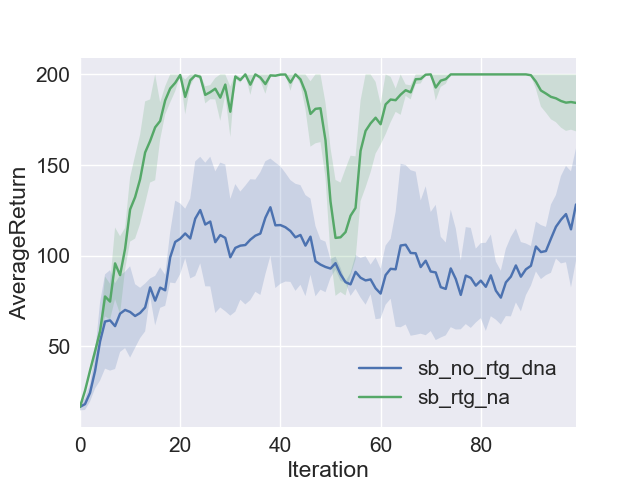
\includegraphics[width=\linewidth]{comparison_sb_with_without_rtg.png}
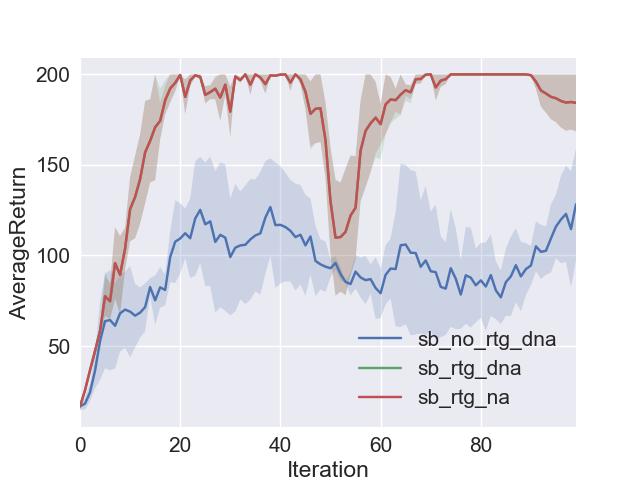
\includegraphics[width=\linewidth]{comparison_average_return_sb.png}


\item In the second graph, compare the learning curves for the experiments prefixed with \verb|lb_|. (The large batch experiments.)


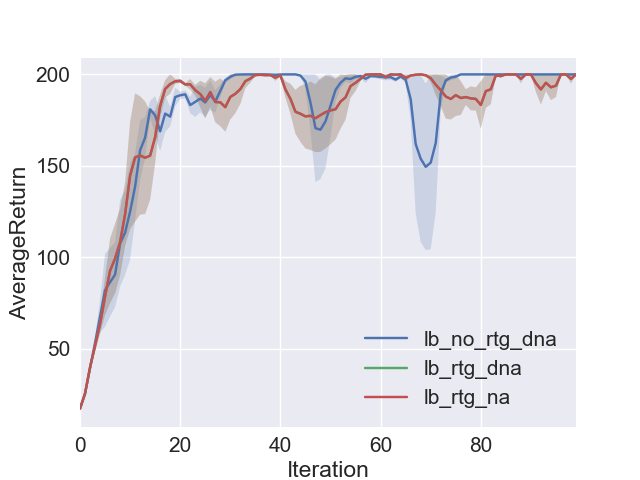
\includegraphics[width=\linewidth]{comparison_average_return_lb.png}
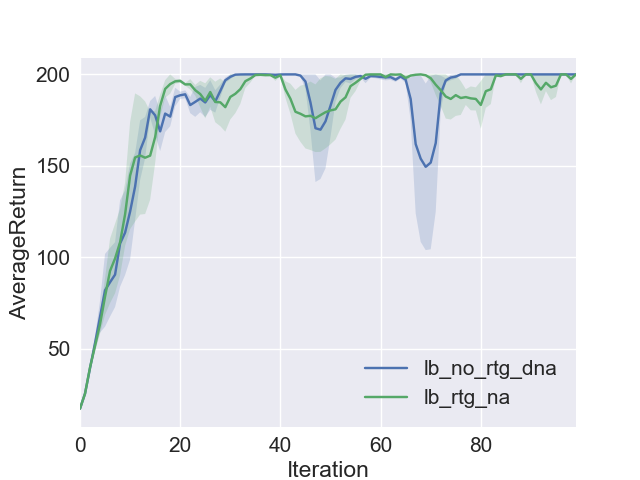
\includegraphics[width=\linewidth]{comparison_average_return_lb(2).png}

\end{itemize}
\item Answer the following questions briefly: 
\begin{itemize}
\item Which gradient estimator has better performance without advantage-centering---the trajectory-centric one, or the one using reward-to-go? 

\begin{solution}
The reward-to-go has clearly better performances as we can see on the graph. This is obvious for small batches, a bit less for large ones.
\end{solution}

\item Did advantage centering help?

\begin{solution}
We can see on the graphs that advantage centering helped. The variance is indeed decreased.
\end{solution}

\item Did the batch size make an impact?
\begin{solution}
The batch size did have an impact. As we can see, for small batches without reward-to-go, the average return remains beneath 150, even for 100 iterations. Overall, the variance is pretty high. 
For large batches, the biggest difference is the improvement for experiments without reward-to-go, as they reach the max average return after only 20 iterations. The variance is also drastically reduced for this experiment. Concerning the experiments implementing the reward-to-go, increasing the batch size avoided that peak of low returns at around 50 iterations. The algorithm is more robust.
\end{solution}

\end{itemize}
\item Provide the exact command line configurations you used to run your experiments. (To verify batch size, learning rate, architecture, and so on.)

\begin{lstlisting}
python train_pg_f18.py CartPole-v0 -n 180 -b 1000 -e 3 -dna  --exp_name sb_no_rtg_dna

python train_pg_f18.py CartPole-v0 -n 150 -b 1000 -e 3 -dna -lr 0.01 --exp_name sb_no_rtg_dna
\end{lstlisting}
\graphicspath{ {./../figures/} }
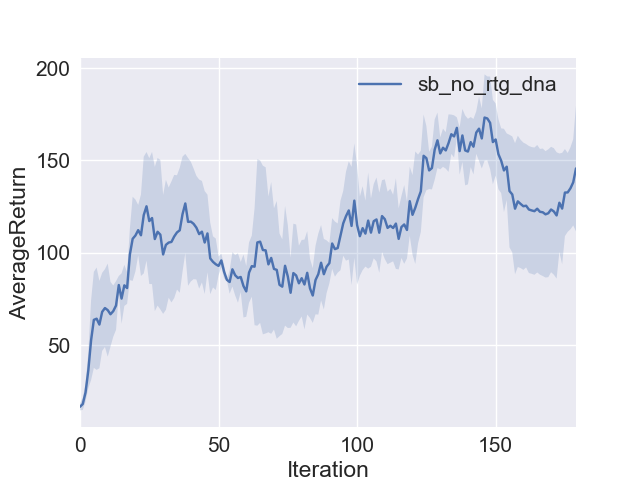
\includegraphics{sb_no-rtg_dna_180-iter.png}
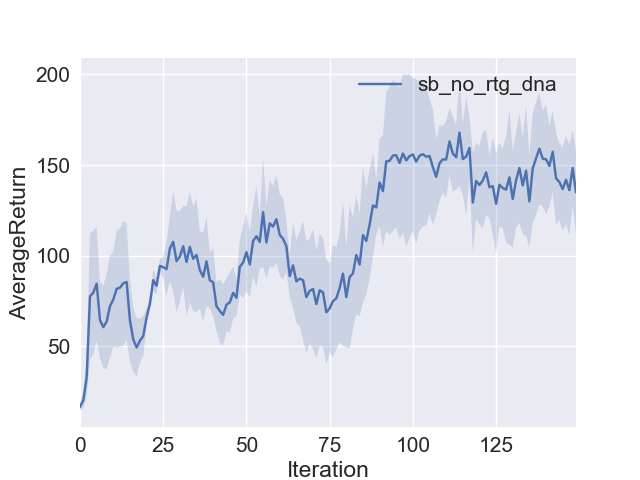
\includegraphics{sb_no-rtg_dna_150-iter_lr-0,01.png}



To check wether with small batches and no reward-to-go, the cartpole reaches the max average return: 
$python train_pg_f18.py CartPole-v0 -n 130 -b 1000 -e 3 -dna  --exp_name sb_no_rtg_dna$


\end{itemize}

\textbf{What to Expect:}
\begin{itemize}
\item The best configuration of CartPole in both the large and small batch cases converge to a maximum score of 200.
\end{itemize}


\textbf{Problem 5. InvertedPendulum:} Run experiments in \verb|InvertedPendulum-v2| continuous control environment as follows:
\begin{lstlisting}
python train_pg_f18.py InvertedPendulum-v2 -ep 1000 --discount 0.9 -n 100 -e 3 -l 2 -s 64 -b <b*> -lr <r*> -rtg --exp_name hc_b<b*>_r<r*>
\end{lstlisting}
where your task is to find the smallest batch size \texttt{b*} and largest learning rate \texttt{r*} that gets to optimum (maximum score of 1000) in less than 100 iterations. The policy performance may fluctuate around 1000 -- this is fine. The precision of \texttt{b*} and \texttt{r*} need only be one significant digit.

\textbf{Deliverables:}

\begin{itemize}
\item Given the \texttt{b*} and \texttt{r*} you found, provide a learning curve where the policy gets to optimum (maximum score of ~1000) in less than 100 iterations. (This may be for a single random seed, or averaged over multiple.)
\item Provide the exact command line configurations you used to run your experiments.
\end{itemize}


\section{Implement Neural Network Baselines}
For the rest of the assignment we will use ``reward-to-go.''

\textbf{Problem 6. Neural network baseline:} We will now implement a value function as a state-dependent neural network baseline. The sections in the code are marked by ``Problem 6.''
\begin{enumerate} [label=(\alph*)]
    \item In \verb|Agent.build_computation_graph| implement $V_\phi^\pi$, a neural network that predicts the expected return conditioned on a state. Also implement the loss function to train this network and its update operation \texttt{self.baseline\_op}.
    \item In \verb|Agent.compute_advantage|, use the neural network to predict the expected state-conditioned return (use the session to call \texttt{self.baseline\_prediction}), normalize it to match the statistics of the current batch of ``reward-to-go'', and subtract this value from the ``reward-to-go'' to yield an estimate of the advantage. This implements $\left(\sum_{t'=t}^T \gamma^{t'-t} r(s_{it'}, a_{it'})\right) - V_\phi^\pi\left(s_{it}\right)$.
    \item In \verb|Agent.update_parameters|, update the parameters of the the neural network baseline by using the Tensorflow session to call \texttt{self.baseline\_op}. ``Rescale'' the target values for the neural network baseline to have a mean of zero and a standard deviation of one.
\end{enumerate}

\section{More Complex Tasks}
\textbf{Note:} The following tasks would take quite a bit of time to train. Please start early!

\textbf{Problem 7: LunarLander} For this problem, you will use your policy gradient implementation to solve \verb|LunarLanderContinuous-v2|.
Use an episode length of 1000. The purpose of this problem is to help you debug your baseline implementation.
Run the following command:
\begin{lstlisting}
python train_pg_f18.py LunarLanderContinuous-v2 -ep 1000 --discount 0.99 -n 100 -e 3 -l 2 -s 64 -b 40000 -lr 0.005 -rtg --nn_baseline --exp_name ll_b40000_r0.005
\end{lstlisting}
\textbf{Deliverables:}
\begin{itemize}
    \item Plot a learning curve for the above command. You should expect to achieve an average return of around 180.
\end{itemize}
\graphicspath{ {./../figures/} }
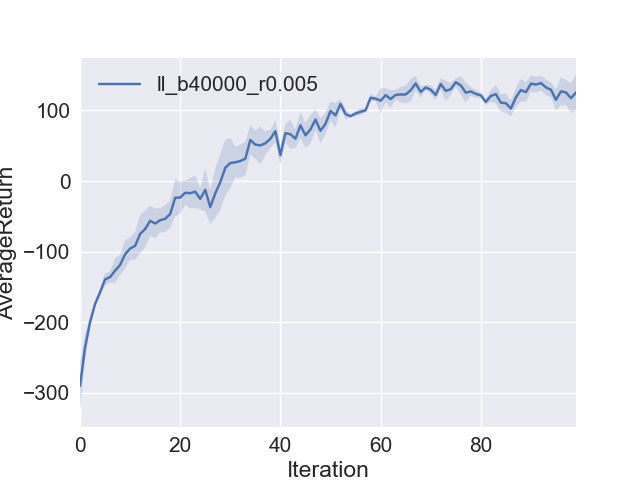
\includegraphics{LunarLander.png}


\textbf{Problem 8: HalfCheetah} For this problem, you will use your policy gradient implementation to solve \verb|HalfCheetah-v2|. 
Use an episode length of 150, which is shorter than the default of 1000 for HalfCheetah (which would speed up your training significantly).
Search over batch sizes \texttt{b} $\in [10000,30000,50000]$ and learning rates \texttt{r} $\in [0.005, 0.01, 0.02]$ to replace \texttt{<b>} and \texttt{<r>} below:
\begin{lstlisting}
python train_pg_f18.py HalfCheetah-v2 -ep 150 --discount 0.9 -n 100 -e 3 -l 2 -s 32 -b <b> -lr <r> -rtg --nn_baseline --exp_name hc_b<b>_r<r>
\end{lstlisting}
\textbf{Deliverables:}
\begin{itemize}
    \item How did the batch size and learning rate affect the performance?
    \item Once you've found suitable values of \texttt{b} and \texttt{r} among those choices (let's call them \texttt{b*} and \texttt{r*}), use \texttt{b*} and \texttt{r*}
and run the following commands (remember to replace the terms in the angle brackets):
\begin{lstlisting}
python train_pg_f18.py HalfCheetah-v2 -ep 150 --discount 0.95 -n 100 -e 3 -l 2 -s 32 -b <b*> -lr <r*> --exp_name hc_b<b*>_r<r*>
python train_pg_f18.py HalfCheetah-v2 -ep 150 --discount 0.95 -n 100 -e 3 -l 2 -s 32 -b <b*> -lr <r*> -rtg --exp_name hc_b<b*>_r<r*>
python train_pg_f18.py HalfCheetah-v2 -ep 150 --discount 0.95 -n 100 -e 3 -l 2 -s 32 -b <b*> -lr <r*> --nn_baseline --exp_name hc_b<b*>_r<r*>
python train_pg_f18.py HalfCheetah-v2 -ep 150 --discount 0.95 -n 100 -e 3 -l 2 -s 32 -b <b*> -lr <r*> -rtg --nn_baseline --exp_name hc_b<b*>_r<r*>
\end{lstlisting}
The run with reward-to-go and the baseline should achieve an average score close to 200. Provide a single plot plotting the learning curves for all four runs.

\textcolor{red}{NOTE: In an earlier version of the homework (before 9/13/18) we had the discount as 0.9, in which case the run with reward-to-go and baseline should achieve an average score close to 150, and there would not be much difference between the runs with reward-to-go (with or without baseline). If you have already done this part with a discount of 0.9, you do not need to redo the problem, but you would then expect the best scoring run to be about 150 rather than 200.}
\end{itemize}


\section{Bonus!}

Choose any (or all) of the following:
\begin{itemize}
\item A serious bottleneck in the learning, for more complex environments, is the sample collection time. In \verb|train_pg_f18.py|, we only collect trajectories in a single thread, but this process can be fully parallelized across threads to get a useful speedup. Implement the parallelization and report on the difference in training time. 
\item Implement GAE-$\lambda$ for advantage estimation.\footnote{\url{https://arxiv.org/abs/1506.02438}} Run experiments in a MuJoCo gym environment to explore whether this speeds up training. (\verb|Walker2d-v1| may be good for this.)
\item In PG, we collect a batch of data, estimate a single gradient, and then discard the data and move on. Can we potentially accelerate PG by taking multiple gradient descent steps with the same batch of data? Explore this option and report on your results. Set up a fair comparison between single-step PG and multi-step PG on at least one MuJoCo gym environment. 
\end{itemize}

\section{Submission}
Your report should be a document containing 
\begin{enumerate} [label=(\alph*)]
\item 
Your mathematical response (written in \LaTeX) for Problem 1.
\item All graphs requested in Problems 4, 5, 7, and 8.
\item Answers to short explanation questions in section 5 and 7.
\item All command-line expressions you used to run your experiments.
\item (Optionally) Your bonus results (command-line expressions, graphs, and a few sentences that comment on your findings).
\end{enumerate}

Please also submit your modified \verb|train_pg_f18.py| file. If your code includes additional files, provide a zip file including your \verb|train_pg_f18.py| and all other files needed to run your code. Please include a \verb|README.md| with instructions needed to exactly duplicate your results (including command-line expressions).

Turn in your assignment by September 19th 11:59pm on Gradescope. Uploade the zip file with your code to \textbf{HW2 Code}, and upload  the PDF of your report to \textbf{HW2}.
\end{document}


